\documentclass[12pt, letterpaper]{article}
\usepackage[margin=1in]{geometry}
\usepackage[T1]{fontenc}
\usepackage{lmodern}
\usepackage{cmap}
\usepackage[utf8]{inputenc}
\usepackage{amsmath, amssymb, amsthm}
\usepackage{mathtools}
\usepackage{enumitem}
\usepackage{booktabs}
\usepackage{xcolor}
\usepackage{titlesec}
\usepackage{parskip}
\usepackage{hyperref}
\usepackage{fancyhdr}
\usepackage{tcolorbox}
\usepackage{graphicx}
\usepackage{caption}
\tcbuselibrary{skins, breakable}

\definecolor{darkblue}{RGB}{15,55,115}
\definecolor{midblue}{RGB}{30,100,180}
\definecolor{theorybg}{RGB}{245,250,255}
\definecolor{questionbg}{RGB}{255,252,240}
\definecolor{evencolor}{RGB}{60,0,100}

\hypersetup{colorlinks=true,linkcolor=darkblue,urlcolor=midblue,
  pdftitle={Ljungqvist \& Sargent --- Recursive Macroeconomic Theory --- Complete Solutions, Chapter 7}}

\setlength{\headheight}{14pt}
\pagestyle{fancy}
\fancyhf{}
\renewcommand{\headrulewidth}{0.4pt}
\fancyhead[L]{\small\textcolor{darkblue}{\textit{Ljungqvist \& Sargent --- Recursive Macroeconomic Theory}}}
\fancyhead[R]{\small\textcolor{darkblue}{\thepage}}
\fancyfoot[C]{\small\textcolor{gray}{Complete Solutions --- Chapter 7}}

\titleformat{\section}[block]
  {\large\bfseries\color{darkblue}}{}{0pt}{}
  [\vspace{2pt}\color{darkblue}\rule{\textwidth}{1.5pt}\vspace{4pt}]

\titleformat{\subsection}[block]
  {\normalsize\bfseries\color{midblue}}{}{0pt}{}
  [\vspace{1pt}\color{midblue}\rule{0.5\textwidth}{0.8pt}\vspace{3pt}]

\tcbset{
  theorybox/.style={
    enhanced,breakable,colback=theorybg,colframe=darkblue,
    fonttitle=\bfseries\small, coltitle=white,boxrule=0.5pt,arc=3pt,
    left=6pt,right=6pt,top=4pt,bottom=4pt,title={Key Theory},
  },
  questionbox/.style={
    enhanced,breakable,colback=questionbg,colframe=gray!60,
    fonttitle=\bfseries\small\color{gray!60!black},boxrule=0.4pt,arc=2pt,
    left=6pt,right=6pt,top=4pt,bottom=4pt,title={\textit{Question}},
  },
  oddbox/.style={
    enhanced,breakable,colback=white,colframe=darkblue,
    attach boxed title to top left={yshift=-2mm,xshift=6mm},
    boxed title style={colback=darkblue,colframe=darkblue,arc=2pt,
      boxrule=0pt,left=6pt,right=6pt,top=3pt,bottom=3pt},
    fonttitle=\bfseries\large\color{white},
    boxrule=0.8pt,arc=3pt,
    left=8pt,right=8pt,top=10pt,bottom=6pt,
  },
  evenbox/.style={
    enhanced,breakable,colback=white,colframe=evencolor,
    attach boxed title to top left={yshift=-2mm,xshift=6mm},
    boxed title style={colback=evencolor,colframe=evencolor,arc=2pt,
      boxrule=0pt,left=6pt,right=6pt,top=3pt,bottom=3pt},
    fonttitle=\bfseries\large\color{white},
    boxrule=0.8pt,arc=3pt,
    left=8pt,right=8pt,top=10pt,bottom=6pt,
  },
  databox/.style={
    enhanced,breakable,colback=gray!8,colframe=gray!55,
    fonttitle=\bfseries\small\color{gray!60!black},boxrule=0.4pt,arc=2pt,
    left=6pt,right=6pt,top=4pt,bottom=4pt,title={Numerical exercise --- see the companion code},
  },
  trapbox/.style={
    enhanced,breakable,colback=red!4,colframe=red!45!black,
    fonttitle=\bfseries\small\color{white},boxrule=0.4pt,arc=2pt,
    coltitle=white,
    left=6pt,right=6pt,top=4pt,bottom=4pt,title={Where this goes wrong},
  },
}

\newcommand{\pd}[2]{\dfrac{\partial #1}{\partial #2}}
\newcommand{\dd}[2]{\dfrac{d #1}{d #2}}
\newcommand{\MRS}{\mathrm{MRS}}
\newcommand{\MRT}{\mathrm{MRT}}
\newcommand{\MU}{\mathrm{MU}}
\newcommand{\Var}{\mathrm{Var}}
\newcommand{\Cov}{\mathrm{Cov}}
\newcommand{\E}{\mathrm{E}}
\newcommand{\MPK}{\mathrm{MPK}}
\newcommand{\MPL}{\mathrm{MPL}}
\newcommand{\stst}{^{\ast}}

\setlist[enumerate,1]{label=(\alph*),itemsep=6pt,parsep=2pt}
\setlist[enumerate,2]{label=(\roman*),itemsep=3pt}


\newcommand{\tr}{\operatorname{trace}}

\begin{document}

%======================================================================
% TITLE PAGE
%======================================================================
\begin{titlepage}
\centering
\vspace*{2.5cm}
{\Huge\bfseries\color{darkblue} Recursive Macroeconomic Theory\par}
\vspace{6pt}
{\large Lars Ljungqvist \& Thomas J. Sargent (4th ed., 2018)\par}
\vspace{1.4cm}
{\LARGE\bfseries Complete Solutions\par}
\vspace{6pt}
{\LARGE\bfseries Chapter 7 --- Recursive Competitive Equilibrium: I\par}
\vspace{1.2cm}
{\large All 7 end-of-chapter exercises, 7.1--7.7 (pp.~244--248)\par}
\vspace{2cm}

\begin{tcolorbox}[theorybox,title={What is in this file},width=0.86\textwidth]
\small
Exercises 7.1--7.5 are one industry seen five ways: a price-taking firm with arbitrary beliefs
(7.1), the same firm with rational expectations (7.2), a planner (7.3), a monopolist (7.4) and a
duopoly (7.5). All are linear regulators, solved with the program of Exercise~5.1(b)
(\texttt{olrp}, Python instead of Matlab) and, for the duopoly, a Python \texttt{nnash}. Exercises
7.6 (time-inconsistent preferences) and 7.7 (equilibrium search) are conceptual; each gets a worked
numerical illustration with parameters stated where it is used.

\smallskip
The companion notebook \texttt{ls\_ch07.ipynb} (same folder) computes every number quoted here and
checks each one by an independent route with an \texttt{assert}: Riccati iteration vs \texttt{scipy}'s
DARE vs undetermined coefficients; the rational-expectations fixed point vs the planner; \texttt{nnash}
vs best-response iteration; grid solutions vs closed forms.

\smallskip
Question boxes reproduce the full statement. Blue boxes are odd-numbered exercises, purple boxes
even-numbered ones.
\end{tcolorbox}

\vfill
{\small MPE Insper --- Macroeconomia I --- 2026, 3\textordmasculine{} trimestre\par}
\end{titlepage}

\tableofcontents
\newpage

%======================================================================
\section{Chapter 7 \quad Recursive Competitive Equilibrium: I}
%======================================================================

\begin{tcolorbox}[theorybox,title={Chapter 7 Overview}]
\textbf{Big $K$, little $k$.} A price-taking agent's state has two parts: $x$, which it controls,
and $X$, the same variable chosen ``by the market'', which it only forecasts through a
\emph{perceived} law $X'=G(X)$ (7.3.3). Its Bellman equation (7.3.1) gives a rule $u=h(x,X)$
(7.3.5). Setting $x=X$ \emph{after} optimising gives the \emph{actual} law
$X'=G_A(X)\equiv g[X,X,h(X,X)]$ (7.3.6).

\textbf{Recursive competitive (rational expectations) equilibrium} (p.~231): $h$, $G_A$, $G$ such that
$h$ is optimal given $G$ and $G_A=G$. In the adjustment-cost model of section 7.2 the map from
perceived to actual laws is $H\mapsto\mathcal M(H)$, $H(Y)=nh(Y/n,Y)$ (7.2.10), and an equilibrium is
a fixed point of $\mathcal M$. $\mathcal M$ need not be a contraction.

\textbf{Planning shortcut} (section 7.2.1). With $n=1$, the planner who maximises
$\sum\beta^tS_t$, $S_t=\int_0^{Y_t}(A_0-A_1x)dx-.5d(Y_{t+1}-Y_t)^2$ (7.2.11), has Euler equation
(7.2.16), which is the firm's Euler equation (7.2.7) with $y_t=Y_t$. The planner's policy is the
equilibrium law $H$.

\textbf{Markov perfect equilibrium} (sections 7.6--7.7). Without price taking, each player's
Bellman equation takes the rival's \emph{policy} as given (7.6.4)--(7.6.5). In linear-quadratic
games this gives stacked Riccati equations (7.7.4)--(7.7.7), iterated backward to a stationary pair
$(F_1,F_2)$ (the book's \texttt{nnash.m}).

\textbf{The regulator used throughout} (chapter 5): maximise $-\sum_t\beta^t\{x_t'Rx_t+u_t'Qu_t\}$ s.t.\
$x_{t+1}=Ax_t+Bu_t$. The solution is $v(x)=-x'Px$, $u=-Fx$, with
$P=R+\beta A'PA-\beta^2A'PB(Q+\beta B'PB)^{-1}B'PA$ and $F=\beta(Q+\beta B'PB)^{-1}B'PA$.
\end{tcolorbox}

\begin{tcolorbox}[databox,title={Parameter values used in 7.1--7.5 (given in Exercise 7.1(c))}]
$A_0=100$, $A_1=.05$, $\beta=.95$, $d=10$; perceived law in 7.1: $H_0=95.5$, $H_1=.95$.
\end{tcolorbox}

%----------------------------------------------------------------------
\subsection{Competitive Equilibrium with Adjustment Costs}
%----------------------------------------------------------------------

%------- 7.1 -------
\begin{tcolorbox}[oddbox,title={Exercise 7.1 \quad A competitive firm}]
\begin{tcolorbox}[questionbox]
p.~244. A competitive firm seeks to maximize
\[
\sum_{t=0}^\infty\beta^tR_t \tag{1}
\]
where $\beta\in(0,1)$, and time $t$ revenue $R_t$ is
\[
R_t=p_ty_t-.5d\,(y_{t+1}-y_t)^2,\qquad d>0, \tag{2}
\]
where $p_t$ is the price of output, and $y_t$ is the time $t$ output of the firm. Here
$.5d(y_{t+1}-y_t)^2$ measures the firm's cost of adjusting its rate of output. The firm starts with a
given initial level of output $y_0$. The price lies on the market demand curve
\[
p_t=A_0-A_1Y_t,\quad A_0,A_1>0 \tag{3}
\]
where $Y_t$ is the market level of output, which the firm takes as exogenous, and which the firm
believes follows the law of motion
\[
Y_{t+1}=H_0+H_1Y_t, \tag{4}
\]
with $Y_0$ as a fixed initial condition.

\textbf{a.} Formulate the Bellman equation for the firm's problem.

\textbf{b.} Formulate the firm's problem as a discounted optimal linear regulator problem, being
careful to describe all of the objects needed. What is the \emph{state} for the firm's problem?

\textbf{c.} Use the Matlab program \texttt{olrp.m} to solve the firm's problem for the following
parameter values: $A_0=100$, $A_1=.05$, $\beta=.95$, $d=10$, $H_0=95.5$, and $H_1=.95$. Express the
solution of the firm's problem in the form
\[
y_{t+1}=h_0+h_1y_t+h_2Y_t, \tag{5}
\]
giving values for the $h_j$'s.

\textbf{d.} If there were $n$ identical competitive firms all behaving according to equation (5),
what would equation (5) imply for the \emph{actual} law of motion (4) for the market supply $Y$?

\textbf{e.} Formulate the Euler equation for the firm's problem.
\end{tcolorbox}

\textbf{Solution:}

\textbf{(a)} Substitute (3) into (2): $R_t=A_0y_t-A_1Y_ty_t-.5d(y_{t+1}-y_t)^2$. The firm controls
$y_{t+1}$, knows $(y_t,Y_t)$, and forecasts $Y$ with (4). Its Bellman equation is (7.2.5):
\[
\boxed{v(y,Y)=\max_{y'}\Big\{A_0y-A_1Yy-.5d(y'-y)^2+\beta v(y',Y')\Big\}\quad\text{s.t. }Y'=H_0+H_1Y.}
\]

\textbf{(b)} The firm needs $y$ (its own output), $Y$ (to know today's price and forecast tomorrow's)
and a constant (for the intercepts $A_0$, $H_0$). So the \textbf{state} is
$x_t=[\,y_t,\ Y_t,\ 1\,]'$. Take the control to be the change in output, $u_t=y_{t+1}-y_t$. Then
\[
x_{t+1}=\underbrace{\begin{bmatrix}1&0&0\\0&H_1&H_0\\0&0&1\end{bmatrix}}_{A}x_t
+\underbrace{\begin{bmatrix}1\\0\\0\end{bmatrix}}_{B}u_t .
\]
The return must be written as $R_t=-(x_t'Rx_t+u_t'Qu_t)$. With
\[
R=\begin{bmatrix}0&A_1/2&-A_0/2\\A_1/2&0&0\\-A_0/2&0&0\end{bmatrix},\qquad Q=\frac d2,
\]
we get $x'Rx=2\cdot\frac{A_1}{2}yY+2\cdot\big(-\frac{A_0}{2}\big)y=A_1yY-A_0y$ and $u'Qu=.5du^2$, so
$-(x'Rx+u'Qu)=A_0y-A_1Yy-.5du^2=R_t$. \checkmark{} The objects are $(\beta,A,B,R,Q)$; the firm
maximises $-\sum_t\beta^t\{x_t'Rx_t+u_t'Qu_t\}$ given $x_0=[y_0,Y_0,1]'$, with solution
$v(x)=-x'Px$, $u_t=-Fx_t$.

\emph{Remark.} $R$ is not positive semidefinite: revenue is \emph{linear} in $y$. The problem is
still well posed. With $B=e_1$, $B'PB=P_{yy}$ and the $(y,y)$ entry of the Riccati map is
$R_{yy}+\beta P_{yy}-\beta^2(P_{yy})^2/(Q+\beta P_{yy})$. Starting from $P=0$ it stays at
$P_{yy}=0$ at every iteration, so $v$ is linear in $y$. The discounted system is stable because the
roots of $A-BF$ are at most $1<1/\sqrt\beta$.

\textbf{(c)} From $u=-Fx$, $y_{t+1}=y_t+u_t=(1-F_1)y_t-F_2Y_t-F_3$, so $h_0=-F_3$,
$h_1=1-F_1$, $h_2=-F_2$. Iterating the Riccati equation from $P=0$ (\texttt{olrp}, 489 steps) gives
\[
\boxed{y_{t+1}=96.9487+1.0000\,y_t-0.046282\,Y_t,}
\]
\[
P=\begin{bmatrix}0&0.25641&-534.744\\0.25641&-0.07509&163.721\\-534.744&163.721&-358775.96\end{bmatrix}.
\]
Part (e) derives the same numbers in closed form:
$h_1=1$, $h_2=-\beta A_1H_1/[d(1-\beta H_1)]=-.045125/.975=-0.0462821$,
$h_0=\beta(A_0-A_1H_0+dh_2H_0)/[d(1-\beta)]=.95(100-4.775-44.1994)/.5=96.9487$.

\emph{Reading of $h_1=1$.} The firm is a price taker and revenue is linear in $y$, so its own level
of output does not affect how fast it wants to change it. The change $y_{t+1}-y_t=96.95-0.0463Y_t$
depends only on the forecast of prices, i.e.\ on $Y_t$.

\textbf{(d)} With $n$ identical firms, $Y_t=ny_t$ and each firm uses (5). Multiply (5) by $n$:
\[
Y_{t+1}=ny_{t+1}=nh_0+h_1(ny_t)+nh_2Y_t
\quad\Longrightarrow\quad
\boxed{Y_{t+1}=nh_0+(h_1+nh_2)Y_t,}
\]
which is (7.2.10) for this model. So the actual law has $H_0^A=nh_0$ and $H_1^A=h_1+nh_2$. For
$n=1$: $Y_{t+1}=96.9487+0.953718\,Y_t\neq95.5+.95Y_t$. The beliefs of part (c) are \emph{not}
rational: firms that hold them act in a way that falsifies them. (For $n=10$:
$Y_{t+1}=969.487+0.537179\,Y_t$.)

\textbf{(e)} First-order condition for $y'$ in (a): $-d(y'-y)+\beta v_y(y',Y')=0$ (7.2.6). The
envelope (Benveniste--Scheinkman) condition, differentiating (a) with respect to $y$ at the optimum:
$v_y(y,Y)=A_0-A_1Y+d(y'-y)$. Shift it forward one period and substitute:
\[
\boxed{-d(y_{t+1}-y_t)+\beta\big[A_0-A_1Y_{t+1}+d(y_{t+2}-y_{t+1})\big]=0,}
\]
which is (7.2.7). Here $Y_{t+1}=H_0+H_1Y_t$, and the terminal condition is
$\lim_t\beta^ty_tv_y(y_t,Y_t)=0$ (7.2.8).

\emph{Solving it (the closed form used in (c)).} Write $u_t=y_{t+1}-y_t$ and $p_t=A_0-A_1Y_t$.
The Euler equation reads $du_t=\beta p_{t+1}+\beta du_{t+1}$. Its homogeneous part
$d\beta\lambda^2-d(1+\beta)\lambda+d=0$ in $y$ has roots $\lambda=1$ and $\lambda=1/\beta$. The
transversality condition rules out the root $1/\beta$, so we solve forward:
\[
u_t=\frac1d\sum_{j\ge0}\beta^{j+1}p_{t+1+j}.
\]
The firm changes output by the discounted value of all future prices divided by $d$. Under (4),
$Y_{t+1+j}=H_1^{j+1}Y_t+H_0\sum_{i=0}^{j}H_1^i$, so the coefficient of $Y_t$ in $u_t$ is
$-\frac{A_1}{d}\sum_{j\ge0}(\beta H_1)^{j+1}=-\frac{\beta A_1H_1}{d(1-\beta H_1)}=h_2$.

\emph{By undetermined coefficients.} Guess $y_{t+1}=h_0+h_1y_t+h_2Y_t$. Then
$y_{t+2}-y_{t+1}=h_0+(h_1-1)y_{t+1}+h_2Y_{t+1}$. Substitute into (7.2.7) and match coefficients:
\begin{align*}
y_t:&\quad -d(h_1-1)+\beta d(h_1-1)h_1=0\ \Rightarrow\ (h_1-1)(\beta h_1-1)=0\ \Rightarrow\ h_1=1,\\
Y_t:&\quad -dh_2-\beta A_1H_1+\beta dh_2H_1=0\ \Rightarrow\ h_2=-\frac{\beta A_1H_1}{d(1-\beta H_1)},\\
1:&\quad -dh_0+\beta A_0-\beta A_1H_0+\beta dh_0+\beta dh_2H_0=0\\
&\quad\Rightarrow\ h_0=\frac{\beta(A_0-A_1H_0+dh_2H_0)}{d(1-\beta)}.
\end{align*}
(The root $h_1=1/\beta$ violates (7.2.8). With $h_1=1$ the $y_{t+1}$ terms cancel: $y_{t+2}-y_{t+1}=h_0+h_2Y_{t+1}$.)

\begin{tcolorbox}[databox]
\texttt{olrp}, \texttt{scipy}'s DARE and the closed form agree to $10^{-9}$. The quadratic form
matches $R_t$ at random points. The Euler residual of (7.2.7) along a 60-period path generated by
(5) and (4) is $6\times10^{-11}$. The computed $P$ has $P_{yy}=0$ exactly.
\end{tcolorbox}
\end{tcolorbox}

%------- 7.2 -------
\begin{tcolorbox}[evenbox,title={Exercise 7.2 \quad Rational expectations}]
\begin{tcolorbox}[questionbox]
p.~245. Now assume that the firm in problem 1 is ``representative.'' We implement this idea by
setting $n=1$. In equilibrium, we will require that $y_t=Y_t$, but we don't want to impose this
condition at the stage that the firm is optimizing (because we want to retain competitive behavior).
Define a rational expectations equilibrium to be a pair of numbers $H_0,H_1$ such that if the
representative firm solves the problem ascribed to it in problem 1, then the firm's optimal behavior
given by equation (5) implies that $y_t=Y_t\ \forall\,t\ge0$.

\textbf{a.} Use the program that you wrote for exercise \textit{7.1} to determine which if any of the
following pairs $(H_0,H_1)$ is a rational expectations equilibrium: (i) $(94.0888,\ .9211)$;
(ii) $(93.22,\ .9433)$, and (iii) $(95.08187459215024,\ .95245906270392)$?

\textbf{b.} Describe an iterative algorithm that uses the program that you wrote for exercise
\textit{7.1} to compute a rational expectations equilibrium. (You are not being asked actually to use
the algorithm you are suggesting.)
\end{tcolorbox}

\textbf{Solution:}

\textbf{(a)} By 7.1(d) with $n=1$, beliefs $H=(H_0,H_1)$ lead to the actual law
$\mathcal M(H)=\big(h_0(H),\ h_1(H)+h_2(H)\big)$. We need $y_t=Y_t$ for all $t$ when $y_0=Y_0$. By
induction this holds iff $h_0+h_1Y+h_2Y=H_0+H_1Y$ for all $Y$, i.e.\ iff $\mathcal M(H)=H$. Running
the program of 7.1 at each candidate:
\medskip

\begin{center}
\begin{tabular}{@{}lccc@{}}
\toprule
& perceived $(H_0,H_1)$ & actual $(h_0,\ h_1+h_2)$ & REE? \\
\midrule
(i) & $(94.0888,\ .9211)$ & $(118.46676,\ 0.9649856)$ & no \\
(ii) & $(93.22,\ .9433)$ & $(104.73644,\ 0.9568606)$ & no \\
(iii) & $(95.081875,\ .952459)$ & $(95.081875,\ 0.952459)$ & \textbf{yes} \\
\bottomrule
\end{tabular}
\end{center}
Only \textbf{(iii)} is a rational expectations equilibrium; its gap is $1.3\times10^{-10}$, which is
the tolerance of the Riccati iteration.

\emph{Closed form (independent check).} Use the formulas of 7.1(e). The slope condition
$H_1=1+h_2(H_1)$ reads
\[
\begin{gathered}
H_1-1=-\frac{\beta A_1H_1}{d(1-\beta H_1)}
\ \Longleftrightarrow\ d(H_1-1)(1-\beta H_1)+\beta A_1H_1=0\\
\Longleftrightarrow\ d\beta H_1^2-[d(1+\beta)+\beta A_1]H_1+d=0 .
\end{gathered}
\]
With our numbers this is $9.5H_1^2-19.5475H_1+10=0$. The roots are $0.95245906$ and $1.10517$;
their product is $1/\beta$. The stable root is $H_1=0.95245906270392$. The intercept condition
$H_0=h_0(H_0,H_1)$ with $dh_2=d(H_1-1)$ gives
\[
\begin{gathered}
H_0d(1-\beta)=\beta\big[A_0-A_1H_0-d(1-H_1)H_0\big]
\ \Longrightarrow\
H_0=\frac{\beta A_0}{d(1-\beta)+\beta A_1+\beta d(1-H_1)},\\
H_0=\frac{95}{0.5+0.0475+0.4516389}=95.0818746 .
\end{gathered}
\]
The implied steady state is $H_0/(1-H_1)=2000=A_0/A_1$. There the price is \emph{zero}: with no
production cost other than adjustment, a steady state needs $u=0$, and by the forward solution of
7.1(e) that requires $\sum\beta^jp=0$.

\textbf{(b)} \emph{Algorithm (iterate on the map from perceived to actual laws).}
\begin{enumerate}[label=\arabic*.]
\item Guess $H^{(0)}=(H_0^{(0)},H_1^{(0)})$, e.g.\ $(95.5,.95)$; choose a relaxation weight
$\gamma\in(0,1]$ and a tolerance $\varepsilon$.
\item Given $H^{(j)}$, build $(A,B,R,Q)$ of 7.1(b) with $(H_0,H_1)=H^{(j)}$. Solve it with the
program of 7.1 and read off $(h_0,h_1,h_2)$.
\item Form the actual law $\mathcal M(H^{(j)})=(nh_0,\ h_1+nh_2)$ with $n=1$.
\item Update $H^{(j+1)}=(1-\gamma)H^{(j)}+\gamma\,\mathcal M(H^{(j)})$.
\item Stop when $\|H^{(j+1)}-H^{(j)}\|<\varepsilon$; then $H^{(j+1)}$ is (approximately) an REE.
Otherwise return to step 2.
\end{enumerate}
\emph{Why the relaxation $\gamma$.} $\mathcal M$ is not a contraction in general (footnote 5,
p.~228). Near the fixed point its Jacobian is triangular, because $h_1+h_2$ does not depend on $H_0$.
The diagonal entries are
\[
\frac{\partial h_0}{\partial H_0}=\frac{\beta(-A_1+dh_2)}{d(1-\beta)}=\frac{\beta[-A_1-d(1-H_1)]}{d(1-\beta)}=-0.99828,
\]
\[
\frac{\partial(1+h_2)}{\partial H_1}=-\frac{\beta A_1}{d(1-\beta H_1)^2}=-0.52451 .
\]
With $\gamma=1$ the error in $H_0$ shrinks by the factor $0.998$ per step and flips sign each time,
so convergence is extremely slow. With $\gamma=.5$ the eigenvalues become $1-\gamma+\gamma\lambda$,
i.e.\ $0.0009$ and $0.238$, and convergence is fast. Part (b) does not ask for this, but running the
algorithm confirms it: after 150 steps from $(95.5,.95)$ the error is $3.4$ with $\gamma=1$ and
$9\times10^{-11}$ with $\gamma=.5$.

\begin{center}
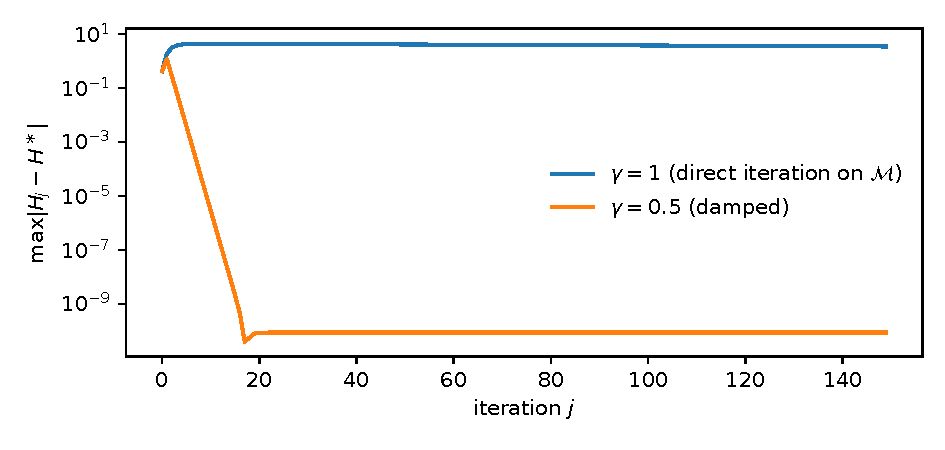
\includegraphics[width=0.8\linewidth]{fig/ls07_ree_iteration.pdf}\\[3pt]
\captionof{figure}{Exercise 7.2(b). Distance to the REE by iteration on the map from perceived to
actual laws. Each step calls the 7.1 program once.}
\end{center}

\begin{tcolorbox}[databox]
The fixed point from the quadratic equals pair (iii) to $10^{-10}$. Central finite differences of
$\mathcal M$ (each evaluation one \texttt{olrp} call) match the two closed-form Jacobian entries to
$10^{-5}$.
\end{tcolorbox}
\end{tcolorbox}

%------- 7.3 -------
\begin{tcolorbox}[oddbox,title={Exercise 7.3 \quad Maximizing welfare}]
\begin{tcolorbox}[questionbox]
p.~246. A planner seeks to maximize the welfare criterion
\[
\sum_{t=0}^\infty\beta^tS_t, \tag{1}
\]
where $S_t$ is ``consumer surplus plus producer surplus'' defined to be
\[
S_t=S(Y_t,Y_{t+1})=\int_0^{Y_t}(A_0-A_1x)\,dx-.5d\,(Y_{t+1}-Y_t)^2 .
\]
\textbf{a.} Formulate the planner's Bellman equation.

\textbf{b.} Formulate the planner's problem as an optimal linear regulator, and, for the same
parameter values in exercise 7.1, solve it using the Matlab program \texttt{olrp.m}. Represent the
solution in the form $Y_{t+1}=s_0+s_1Y_t$.

\textbf{c.} Compare your answer in part b with your answer to part a of exercise \textit{7.2}.
\end{tcolorbox}

\textbf{Solution:}

\textbf{(a)} $\int_0^{Y}(A_0-A_1x)dx=A_0Y-\frac{A_1}{2}Y^2$. The only state is $Y$; the planner
chooses $Y'$. The Bellman equation is (7.2.13):
\[
\boxed{V(Y)=\max_{Y'}\Big\{A_0Y-\frac{A_1}{2}Y^2-.5d(Y'-Y)^2+\beta V(Y')\Big\}.}
\]

\textbf{(b)} State $x_t=[Y_t,\ 1]'$, control $u_t=Y_{t+1}-Y_t$, $A=I_2$, $B=[1,0]'$,
\[
R=\begin{bmatrix}A_1/2&-A_0/2\\-A_0/2&0\end{bmatrix},\qquad Q=\frac d2 .
\]
Check: $x'Rx=\frac{A_1}{2}Y^2-A_0Y$, so $-(x'Rx+u'Qu)=A_0Y-\frac{A_1}{2}Y^2-.5du^2=S_t$.
\checkmark{} Then $Y_{t+1}=(1-F_1)Y_t-F_2$. \texttt{olrp} (496 steps) gives
\[
\boxed{Y_{t+1}=95.08187459215+0.95245906270392\,Y_t,}\qquad
P=\begin{bmatrix}0.2627&-525.409\\-525.409&-949181.25\end{bmatrix}.
\]

\textbf{(c)} $(s_0,s_1)$ is \emph{identical} to pair (iii) of 7.2(a), the rational expectations
equilibrium. The reason is the argument of section 7.2.1. The first-order condition of (a) is
$-d(Y'-Y)+\beta V'(Y')=0$, and the envelope condition is $V'(Y)=A_0-A_1Y+d(Y'-Y)$. Combining them:
\[
\beta A_0+dY_t-[\beta A_1+d(1+\beta)]Y_{t+1}+d\beta Y_{t+2}=0 \qquad(7.2.16).
\]
Setting $y_t=Y_t$ in the firm's Euler equation (7.2.7) gives the same equation:
$-dY_{t+1}+dY_t+\beta A_0-\beta A_1Y_{t+1}+\beta dY_{t+2}-\beta dY_{t+1}=0$. Its characteristic
polynomial $d\beta z^2-[\beta A_1+d(1+\beta)]z+d$ is the quadratic of 7.2(a). The stable root is
$s_1=H_1$, and the steady state $Y=A_0/A_1$ gives $s_0=(1-s_1)A_0/A_1=H_0$. The competitive
equilibrium is efficient; this is the first welfare theorem, and the equilibrium price
$p_t=A_0-A_1Y_t$ is the planner's shadow price of output.

\begin{tcolorbox}[databox]
$S_t$ by numerical quadrature equals the quadratic form at random points. \texttt{olrp} and DARE
agree to $10^{-8}$, and $(s_0,s_1)$ equals the 7.2 closed form to $10^{-8}$.
\end{tcolorbox}
\end{tcolorbox}

%----------------------------------------------------------------------
\subsection{Market Power: Monopoly and Duopoly}
%----------------------------------------------------------------------

%------- 7.4 -------
\begin{tcolorbox}[evenbox,title={Exercise 7.4 \quad Monopoly}]
\begin{tcolorbox}[questionbox]
p.~246. A monopolist faces the industry demand curve (3) and chooses $Y_t$ to maximize
$\sum_{t=0}^\infty\beta^tR_t$ where $R_t=p_tY_t-.5d(Y_{t+1}-Y_t)^2$ and where $Y_0$ is given.

\textbf{a.} Formulate the firm's Bellman equation.

\textbf{b.} For the parameter values listed in exercise \textit{7.1}, formulate and solve the firm's
problem using \texttt{olrp.m}.

\textbf{c.} Compare your answer in part b with the answer you obtained to part b of exercise
\textit{7.3}.
\end{tcolorbox}

\textbf{Solution:}

\textbf{(a)} The monopolist knows that its own output sets the price: $p_tY_t=A_0Y_t-A_1Y_t^2$.
There is no aggregate variable to forecast, hence no perceived law:
\[
\boxed{V(Y)=\max_{Y'}\Big\{A_0Y-A_1Y^2-.5d(Y'-Y)^2+\beta V(Y')\Big\}.}
\]

\textbf{(b)} This is the planner's regulator of 7.3(b) with $A_1/2$ replaced by $A_1$:
$x=[Y,1]'$, $u=Y'-Y$, $A=I_2$, $B=[1,0]'$, $Q=d/2$,
\[
R=\begin{bmatrix}A_1&-A_0/2\\-A_0/2&0\end{bmatrix}\quad(x'Rx=A_1Y^2-A_0Y).
\]
\texttt{olrp} gives
\[
\boxed{Y_{t+1}=73.472944+0.926527\,Y_t,}\qquad
P=\begin{bmatrix}0.41736&-417.365\\-417.365&-582635.28\end{bmatrix}.
\]
\emph{Check by the Euler equation.} The FOC $-d(Y'-Y)+\beta V'(Y')=0$ and the envelope condition
$V'(Y)=A_0-2A_1Y+d(Y'-Y)$ give
$\beta A_0+dY_t-[2\beta A_1+d(1+\beta)]Y_{t+1}+d\beta Y_{t+2}=0$. The characteristic equation
$9.5z^2-19.595z+10=0$ has roots $0.926527$ and $1.136106$; the stable root is $s_1$. The steady state
solves $A_0-2A_1Y=0$, so $Y=A_0/(2A_1)=1000$ and $s_0=(1-0.926527)\times1000=73.4729$. \checkmark

\textbf{(c)} The monopolist solves the planner's problem with the demand curve replaced by the
\emph{marginal revenue} curve $A_0-2A_1Y$, i.e.\ with slope $2A_1$ instead of $A_1$.
\begin{center}
\begin{tabular}{@{}lccc@{}}
\toprule
& $Y_{t+1}=s_0+s_1Y_t$ & steady-state $Y$ & steady-state $p$ \\
\midrule
planner (= competition, 7.3) & $95.0819+0.952459\,Y_t$ & 2000 & 0 \\
monopoly (7.4) & $73.4729+0.926527\,Y_t$ & 1000 & 50 \\
\bottomrule
\end{tabular}
\end{center}
The monopolist restricts output to half the efficient level and keeps the price at 50. That is a
permanent deadweight loss (footnote 9, p.~238): the market outcome no longer maximises
$\sum\beta^tS_t$. Its adjustment root is smaller ($0.9265<0.9525$), so it moves faster toward a
target that is closer. The steeper marginal-revenue curve raises the cost of being away from the
target relative to the adjustment cost $d$.

\begin{tcolorbox}[databox]
\texttt{olrp}, DARE and the Euler-equation closed form agree to $10^{-8}$.
\end{tcolorbox}
\end{tcolorbox}

%------- 7.5 -------
\begin{tcolorbox}[oddbox,title={Exercise 7.5 \quad Duopoly}]
\begin{tcolorbox}[questionbox]
pp.~246--247. An industry consists of two firms that jointly face the industry-wide inverse demand
curve $p_t=A_0-A_1Y_t$, where now $Y_t=y_{1t}+y_{2t}$. Firm $i=1,2$ maximizes
\[
\sum_{t=0}^\infty\beta^tR_{it} \tag{1}
\]
where $R_{it}=p_ty_{it}-.5d(y_{i,t+1}-y_{it})^2$.

\textbf{a.} Define a Markov perfect equilibrium for this industry.

\textbf{b.} Formulate the Bellman equation for each firm.

\textbf{c.} Use the Matlab program \texttt{nash.m} to compute an equilibrium, assuming the parameter
values listed in exercise \textit{7.1}.
\end{tcolorbox}

\textbf{Solution:} Substituting demand,
$R_{it}=A_0y_{it}-A_1y_{it}^2-A_1y_{it}y_{-i,t}-.5d(y_{i,t+1}-y_{it})^2$ (7.6.3).

\textbf{(a)} Firm $i$'s strategy is a decision rule $y_{i,t+1}=f_i(y_{it},y_{-i,t})$ that depends
only on the payoff-relevant state $(y_{1t},y_{2t})$. A \textbf{Markov perfect equilibrium} is a pair
of value functions $v_1,v_2$ and a pair of policy functions $f_1,f_2$ such that, for $i=1,2$:
(i) given $f_{-i}$, $v_i$ satisfies firm $i$'s Bellman equation in (b) for \emph{every} state
$(y_i,y_{-i})$; and (ii) $f_i(y_i,y_{-i})$ attains the maximum on its right side. ``Markov'' means
that strategies depend on the current state only, not on history. ``Perfect'' means that
optimality holds at all states, including those never reached on the equilibrium path, so the
equilibrium is built by backward induction (p.~239). In the linear-quadratic version sought in (c),
$f_i$ is affine: $u_{it}=-F_ix_t$ with $x_t=[1,y_{1t},y_{2t}]'$ (section 7.7).

\textbf{(b)} For $i=1,2$ (7.6.4)--(7.6.5):
\[
\boxed{\begin{gathered}v_i(y_i,y_{-i})=\max_{y_i'}\Big\{A_0y_i-A_1y_i^2-A_1y_iy_{-i}-.5d(y_i'-y_i)^2+\beta
v_i(y_i',y_{-i}')\Big\}\\ \text{s.t. } y_{-i}'=f_{-i}(y_{-i},y_i).\end{gathered}}
\]
Unlike the competitive firm of 7.1, firm $i$ knows that its rival's next output responds to
$y_i$ through $f_{-i}$, and that its own output moves the price.

\textbf{(c)} Map the game into the form solved by \texttt{nnash} (p.~243). State
$x_t=[1,\ y_{1t},\ y_{2t}]'$, controls $u_{it}=y_{i,t+1}-y_{it}$, law of motion
$x_{t+1}=Ax_t+B_1u_{1t}+B_2u_{2t}$ with $A=I_3$, $B_1=e_2$, $B_2=e_3$. Player $i$ maximises
$-\sum\beta^t\{x_t'R_ix_t+u_{it}'Q_iu_{it}\}$ with $Q_i=d/2$,
\[
R_1=\begin{bmatrix}0&-A_0/2&0\\-A_0/2&A_1&A_1/2\\0&A_1/2&0\end{bmatrix},\qquad
R_2=\begin{bmatrix}0&0&-A_0/2\\0&0&A_1/2\\-A_0/2&A_1/2&A_1\end{bmatrix}.
\]
Check: $x'R_1x=-A_0y_1+A_1y_1^2+A_1y_1y_2$, so $-(x'R_1x+u_1'Q_1u_1)=R_{1t}$. \checkmark{} (The book's
$s_i,w_i,m_i$ are zero here.)

\emph{Algorithm} (7.7.4)--(7.7.7) with discounting. Start from $P_1=P_2=0$. Given $(P_1,P_2)$, the
pair $(F_1,F_2)$ solves the linear system
\[
\begin{gathered}(Q_1+\beta B_1'P_1B_1)F_1+\beta B_1'P_1B_2F_2=\beta B_1'P_1A,\\
\beta B_2'P_2B_1F_1+(Q_2+\beta B_2'P_2B_2)F_2=\beta B_2'P_2A .\end{gathered}
\]
This is (7.7.4) and (7.7.6) written jointly: firm $i$'s best response to $F_{-i}$ in the
one-more-period game. Then update
$P_i\leftarrow R_i+F_i'Q_iF_i+\beta(A-B_1F_1-B_2F_2)'P_i(A-B_1F_1-B_2F_2)$, which is (7.7.5) and
(7.7.7) evaluated at the chosen $F_i$. Iterate until $(P_1,P_2)$ converge. This took 487 steps and gave
\[
F_1=[-65.27422,\ 0.06708,\ 0.02423],\qquad F_2=[-65.27422,\ 0.02423,\ 0.06708],
\]
so that
\[
\boxed{y_{i,t+1}=65.27422+0.93292\,y_{it}-0.02423\,y_{-i,t},\qquad i=1,2.}
\]
The closed-loop matrix $A-B_1F_1-B_2F_2$ has roots $1$ (the constant), $0.95716$ and $0.90869$. The
symmetric steady state is $y_i=65.27422/(1-0.93292+0.02423)=714.90$. Industry output is $1429.80$ and
the price is $28.51$. Starting from $y_{10}=y_{20}$, industry output follows
$Y_{t+1}=130.548+0.908695\,Y_t$.

\emph{Comparison.} Steady-state industry output is $1000$ under monopoly, $1333.3$ under static Cournot
($2A_0/3A_1$), $1429.8$ in the dynamic duopoly and $2000$ under competition. The dynamic duopolists
produce \emph{more} than static Cournot firms. The coefficient $-0.02423$ says that a firm's current
output lowers its rival's next-period output. Output is like a capital stock that deters the rival,
so each firm over-expands to get this strategic effect. The effect is absent from the static game.

\begin{center}
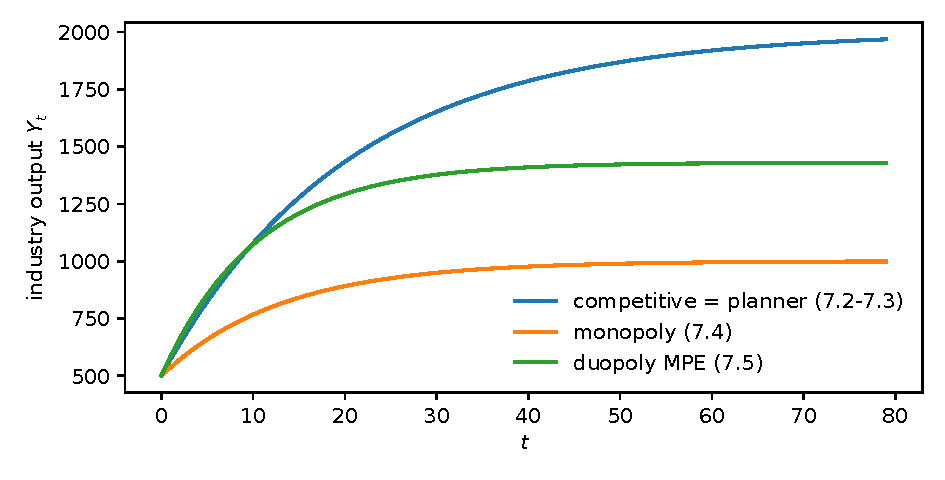
\includegraphics[width=0.85\linewidth]{fig/ls07_market_structures.pdf}\\[3pt]
\captionof{figure}{Exercises 7.2--7.5. Industry output from $Y_0=500$ (duopoly: $y_{i0}=250$).}
\end{center}

\begin{tcolorbox}[databox]
Independent route: best-response iteration. Solve firm 1's infinite-horizon regulator given $F_2$
(state law $A-B_2F_2$, via \texttt{olrp}), then firm 2's given the new $F_1$, and repeat. It
converges in 12 rounds to the \texttt{nnash} pair to $10^{-7}$. \texttt{scipy}'s DARE on firm 1's
problem given $F_2$ returns $F_1$ and $P_1$. The rules are symmetric. The statement names
\texttt{nash.m}; the program supplied with the book is \texttt{nnash.m} (p.~243).
\end{tcolorbox}
\end{tcolorbox}

%----------------------------------------------------------------------
\subsection{Markov Perfection Beyond Linear Games}
%----------------------------------------------------------------------

%------- 7.6 -------
\begin{tcolorbox}[evenbox,title={Exercise 7.6 \quad Self-control}]
\begin{tcolorbox}[questionbox]
p.~247. This is a model of a human who has time inconsistent preferences, of a type proposed by
Phelps and Pollak (1968) and used by Laibson (1994). The human lives from $t=0,\dots,T$. Think of
the human as actually consisting of $T+1$ personalities, one for each period. Each personality is a
distinct agent (i.e., a distinct utility function and constraint set). Personality $T$ has
preferences ordered by $u(c_T)$ and personality $t<T$ has preferences that are ordered by
\[
u(c_t)+\delta\sum_{j=1}^{T-t}\beta^ju(c_{t+j}),
\]
where $u(\cdot)$ is a twice continuously differentiable, increasing, and strictly concave function
of consumption of a single good; $\beta\in(0,1)$, and $\delta\in(0,1]$. When $\delta<1$, preferences
of the sequence of personalities are time inconsistent (that is, not recursive). At each $t$, let
there be a savings technology described by
\[
k_{t+1}+c_t\le f(k_t),
\]
where $f$ is a production function with $f'>0$, $f''\le0$.

\textbf{a.} Define a Markov perfect equilibrium for the $T+1$ personalities.

\textbf{b.} Argue that the Markov perfect equilibrium can be computed by iterating on the following
functional equations:
\begin{align*}
V_{j+1}(k)&=\max_c\{u(c)+\beta\delta W_j(k')\}\\
W_{j+1}(k)&=u[c_{j+1}(k)]+\beta W_j[f(k)-c_{j+1}(k)]
\end{align*}
where $c_{j+1}(k)$ is the maximizer of the right side of the first equation above for $j+1$,
starting from $W_0(k)=u[f(k)]$. Here $W_j(k)$ is the value of
$u(c_{T-j})+\beta u(c_{T-j+1})+\dots+\beta^{T-j}u(c_T)$, taking the decision rules $c_h(k)$ as given
for $h=0,1,\dots,j$.

\textbf{c.} State the optimization problem of the time $0$ person who is given the power to dictate
the choices of all subsequent persons. Write the Bellman equations for this problem. The time $0$
person is said to have a commitment technology for ``self-control'' in this problem.
\end{tcolorbox}

\textbf{Solution:} Index rules by \emph{periods to go}. $c_h(k)$ is the rule of personality
$T-h$, so $c_0$ belongs to personality $T$. This is the indexing the functional equations use.

\emph{Misprint.} The last term of $W_j$ should be $\beta^{j}u(c_T)$, not $\beta^{T-j}u(c_T)$.
$W_j$ starts at date $T-j$, so date $T$ is $j$ periods later. The recursion
$W_{j+1}=u+\beta W_j$ with $W_0=u[f(k)]$ produces exactly $\beta^j$.

\textbf{(a)} The payoff-relevant state at $t$ is $k_t$. A \textbf{Markov perfect equilibrium} is a
collection of consumption rules $\{c_h(k)\}_{h=0}^{T}$, one per personality, with
$0\le c_h(k)\le f(k)$, such that for every $h$ and \emph{every} $k$, $c_h(k)$ maximises personality
$T-h$'s objective
\[
u(c)+\delta\sum_{i=1}^{h}\beta^iu(c_{T-h+i}),
\]
where the future is generated by $k_{T-h+1}=f(k)-c$ and, for $i\ge1$, by the successors' rules:
$c_{T-h+i}=c_{h-i}(k_{T-h+i})$ and $k_{T-h+i+1}=f(k_{T-h+i})-c_{T-h+i}$. Each personality takes its
successors' rules as given (Nash), strategies depend only on $k$ (Markov), and optimality holds at
all $k$, on or off the path (perfect). Personality $T$ has no future, so $c_0(k)=f(k)$.

\textbf{(b)} Backward induction.

\emph{Start.} Personality $T$ consumes everything: $c_0(k)=f(k)$ and $V_0(k)=W_0(k)=u[f(k)]$.

\emph{Step.} Suppose the rules $c_0,\dots,c_j$ of personalities $T,\dots,T-j$ are known, and let
$W_j(k)$ be the $\beta$-discounted utility from date $T-j$ onward that they generate from
$k_{T-j}=k$:
$W_j(k)=\sum_{i=0}^{j}\beta^iu(c_{T-j+i})$. Personality $t=T-j-1$ (with $j+1$ periods to go) values
\[
u(c_t)+\delta\sum_{i=1}^{j+1}\beta^iu(c_{t+i})
=u(c_t)+\delta\beta\sum_{i=0}^{j}\beta^{i}u(c_{T-j+i})
=u(c_t)+\beta\delta\,W_j(k_{t+1}).
\]
The first equality factors out $\delta\beta$ and re-indexes $i\to i+1$. The second uses the fact
that, given the successors' Markov rules, the continuation depends only on $k_{t+1}=f(k)-c_t$.
So personality $t$ solves
\[
V_{j+1}(k)=\max_{c}\{u(c)+\beta\delta W_j(f(k)-c)\},
\]
the first functional equation, and its rule is the maximiser $c_{j+1}(k)$. Now extend $W$ one
period:
\[
\begin{aligned}W_{j+1}(k)&=\sum_{i=0}^{j+1}\beta^iu(c_{T-j-1+i})=u[c_{j+1}(k)]+\beta\sum_{i=0}^{j}\beta^iu(c_{T-j+i})\\
&=u[c_{j+1}(k)]+\beta W_j[f(k)-c_{j+1}(k)],\end{aligned}
\]
the second functional equation. Iterating $j=0,\dots,T-1$ produces every rule. Each is optimal for
its personality at every $k$ given its successors, which is the definition in (a).

\emph{Why two functions.} $V_{j+1}$ is the current personality's own value; it weights tomorrow
by $\beta\delta$. $W_{j+1}$ is how that personality's \emph{predecessors} value the same future; it
weights tomorrow by $\beta$, because $\delta$ is common to all future dates from their viewpoint.
Hence $V_{j+1}(k)=W_{j+1}(k)-\beta(1-\delta)W_j(k')$ at $k'=f(k)-c_{j+1}(k)$. The $W$ update
evaluates $c_{j+1}$; it does \emph{not} maximise. So the envelope theorem does not apply to $W$ and
$W_j$ need not be concave when $\delta<1$. The argmax may then be set-valued and a selection is
needed; the recursion still defines an MPE. With $\delta=1$, $V=W$ and the scheme is ordinary
backward dynamic programming.

\textbf{(c)} With commitment, the time-0 person chooses the whole plan:
\[
\max_{\{c_t,k_{t+1}\}_{t=0}^T}\ u(c_0)+\delta\sum_{t=1}^T\beta^tu(c_t)
\quad\text{s.t.}\quad k_{t+1}+c_t\le f(k_t),\ k_{t+1}\ge0,\ k_0\text{ given}.
\]
Write the objective as $u(c_0)+\delta\beta\big[\sum_{t=1}^{T}\beta^{t-1}u(c_t)\big]$. From date 1 on,
the bracket is an ordinary geometric criterion, so the plan from date 1 is time consistent
\emph{for person 0}. The Bellman equations are, with $J_h$ the value with $h$ periods to go,
\begin{align*}
J_0(k)&=u[f(k)],\\
J_{h+1}(k)&=\max_c\{u(c)+\beta J_h(f(k)-c)\},\qquad h=0,\dots,T-2,\\
V^{c}(k_0)&=\max_{c_0}\{u(c_0)+\beta\delta J_{T-1}(f(k_0)-c_0)\}.
\end{align*}
Only the first step carries $\beta\delta$; every later step uses $\beta$. In the MPE, every
personality applies $\beta\delta$ to its own tomorrow. That is the self-control problem: person 0
would like persons $1,\dots,T-1$ to use $\beta$.

\emph{Worked example} (parameters chosen: $u=\ln c$, $f(k)=\bar Ak^\alpha$, $\bar A=1$,
$\alpha=.36$, $\beta=.96$, $\delta=.6$, $T=10$). Guess $W_j(k)=a_j\ln k+b_j$. $W_0=\ln\bar A+\alpha\ln k$,
so $a_0=\alpha$. Personality with $j+1$ periods to go:
$\max_c\{\ln c+\beta\delta a_j\ln(f-c)\}$. The FOC $1/c=\beta\delta a_j/(f-c)$ gives
\[
c_{j+1}(k)=\frac{f(k)}{1+\beta\delta a_j},\qquad k'=\frac{\beta\delta a_j}{1+\beta\delta a_j}f(k).
\]
Then $W_{j+1}(k)=\ln c+\beta(a_j\ln k'+b_j)=(1+\beta a_j)\ln f(k)+\text{const}$, so
\[
a_{j+1}=\alpha(1+\beta a_j)\ \to\ \frac{\alpha}{1-\alpha\beta}.
\]
The coefficient recursion does not involve $\delta$. With log utility, consumption and savings are
proportional to $f(k)$, so the saving \emph{rate} affects only the constants $b_j$. Commitment gives
$J_h=\tilde a_h\ln k+\dots$ with the same recursion, so $\tilde a_h=a_h$. Hence:
\begin{center}
\begin{tabular}{@{}lcc@{}}
\toprule
saving rate $k_{t+1}/f(k_t)$ at date $t<T$ & MPE & commitment \\
\midrule
$t=0$ & $\dfrac{\beta\delta a_{T-1}}{1+\beta\delta a_{T-1}}$ & same \\[8pt]
$1\le t\le T-1$ & $\dfrac{\beta\delta a_{T-t-1}}{1+\beta\delta a_{T-t-1}}$ & $\dfrac{\beta a_{T-t-1}}{1+\beta a_{T-t-1}}$ \\
\bottomrule
\end{tabular}
\end{center}
Numbers: $a=(0.36,\,0.4844,\,0.5274,\dots,0.5501)$. The MPE saving rates are
$0.2406,0.2406,0.2406,0.2405,0.2403,0.2397,0.2380,0.2330,0.2182,0.1718$ for $t=0,\dots,9$. The
commitment rates are $0.2406,0.3456,0.3456,0.3455,0.3452,0.3445,0.3424,0.3361,0.3174,0.2568$. From
$k_0=.2$, person 0's welfare is $-5.8944$ in the MPE and $-5.7140$ under commitment.

\begin{center}
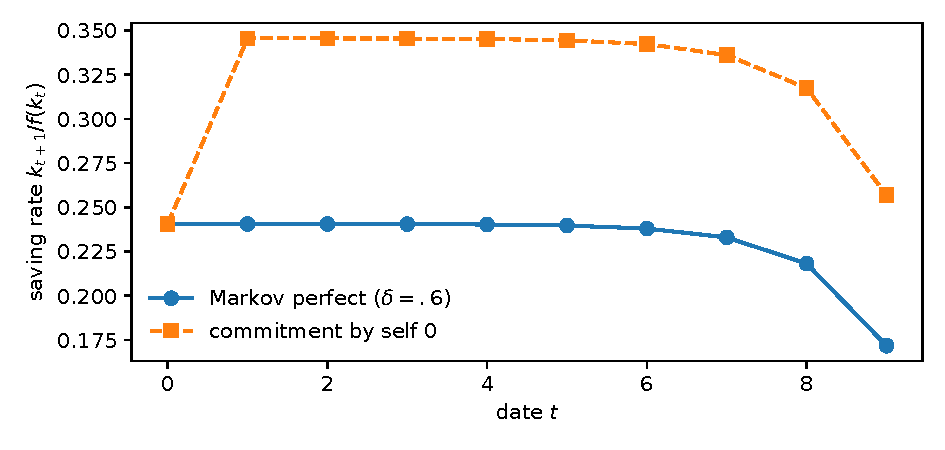
\includegraphics[width=0.8\linewidth]{fig/ls07_selfcontrol.pdf}\\[3pt]
\captionof{figure}{Exercise 7.6. Without commitment each future self saves less than self 0 wants.}
\end{center}

\begin{tcolorbox}[databox]
The functional equations of (b), and the commitment Bellman equations of (c), are iterated on a
120-point grid in $\ln k$. $W_j$ is interpolated by cubic spline and the maximisation is numerical
(bounded scalar search over the saving rate). All saving rates match the closed form to $10^{-6}$ at
every grid point. The notebook also checks that the welfare of self 0 is higher under commitment.
\end{tcolorbox}
\end{tcolorbox}

%------- 7.7 -------
\begin{tcolorbox}[oddbox,title={Exercise 7.7 \quad Equilibrium search}]
\begin{tcolorbox}[questionbox]
p.~248. An economy consists of a continuum of \emph{ex ante} identical workers each of whom is either
employed or unemployed. A worker wants to maximize the expected value of $\sum_{t=0}^\infty\beta^ty_t$
where $\beta\in(0,1)$ and
\[
y_t=\begin{cases}w&\text{if employed}\\ c(U)&\text{if unemployed}.\end{cases}
\]
Each period, an unemployed worker draws one and only one offer to work (until fired) at a wage $w$
drawn from a c.d.f.\ $F(W)=\text{Prob}(w\le W)$ where $F(0)=0$, $F(B)=1$ for $B>0$. Successive draws
from $F$ are i.i.d. If a worker accepts a job, he receives $w$ this period and enters the beginning of
next period as `employed'. At the beginning of each period, each such previously employed worker is
exposed to a probability of $\lambda\in(0,1)$ of being fired; with probability $1-\lambda$ he is not
fired and again receives the previously drawn $w$ as a wage. If fired, the worker becomes newly
unemployed and has the same opportunity as all other unemployed workers, i.e., he draws an offer $w$
from c.d.f.\ $F$. If an unemployed worker rejects that offer, he receives unemployment compensation
$c(U)=c\big[\frac{1}{1+\exp(-6U)}-.5\big]$ and enters next period unemployed. Here $U$ is the
aggregate unemployment rate at the beginning of the period. The unemployment rate tomorrow $U^*$ is
related to the unemployment rate $U$ today by the law of motion
\[
U^*=\lambda(1-U)+(1-\phi(U))U,
\]
where $\phi(U)$ is the fraction of unemployed workers who accept a wage offer this period.

\textbf{a.} Write a Bellman equation for an unemployed worker.

\textbf{b.} Describe the form of an unemployed worker's optimal decision rule.

\textbf{c.} Describe how $\phi(U)$ is implied by a typical worker's optimal decision rule.

\textbf{d.} Define a recursive competitive equilibrium for this environment.
\end{tcolorbox}

\textbf{Solution:} Benefits depend on the aggregate unemployment rate, so a worker must forecast $U$.
This is the ``big $K$, little $k$'' structure of section 7.3. The individual state is employment
status and the wage; the aggregate state is $U$, with perceived law $U'=G(U)$. The model has no
quit option, so an employed worker keeps his wage until fired.

\textbf{(a)} Let $V(U)$ be the value of an unemployed worker at the start of a period, before the
draw, when unemployment is $U$. Let $E(w,U)$ be the value of working this period at wage $w$. A
worker who works this period is fired at the start of next period with probability $\lambda$; he
then draws immediately, so his value is $V(U')$. Hence
\begin{align*}
E(w,U)&=w+\beta\big[(1-\lambda)E(w,G(U))+\lambda V(G(U))\big],\\
\boxed{V(U)}&\boxed{{}=\int_0^B\max\Big\{E(w,U),\ c(U)+\beta V(G(U))\Big\}\,dF(w).}
\end{align*}
The max compares accepting $w$ with rejecting it: collect $c(U)$ and search again next period.

\textbf{(b)} Guess $E(w,U)=w/\kappa+e(U)$ with $\kappa\equiv1-\beta(1-\lambda)$. Substituting,
\[
\frac w\kappa+e(U)=w+\beta(1-\lambda)\frac w\kappa+\beta\big[(1-\lambda)e(G(U))+\lambda V(G(U))\big].
\]
The $w$ terms match because $\frac{w}{\kappa}\big(1-\beta(1-\lambda)\big)=w$. The rest gives
$e(U)=\beta[(1-\lambda)e(G(U))+\lambda V(G(U))]$. So $E$ is strictly increasing in $w$ with slope
$1/\kappa$, while the value of rejecting does not depend on $w$. The optimal rule is therefore a
\textbf{reservation wage} that depends on the aggregate state: accept iff $w\ge\bar w(U)$, where
$E(\bar w(U),U)=c(U)+\beta V(G(U))$:
\[
\boxed{\bar w(U)=\kappa\big[c(U)+\beta V(G(U))-e(U)\big]}
\]
(truncated to $[0,B]$). Substituting $\max\{E,\ c+\beta V'\}=c+\beta V'+\max\{w-\bar w,0\}/\kappa$
into (a) gives
$V(U)=c(U)+\beta V(G(U))+\kappa^{-1}\int_{\bar w(U)}^B(w-\bar w(U))\,dF(w)$. $\bar w$ depends on
$U$ through today's benefit $c(U)$ and, through $G$, on forecasts of future benefits and of future
job values.

\textbf{(c)} All unemployed workers face the same $U$ and use the same $\bar w(U)$. Their offers are
i.i.d., so by the law of large numbers over the continuum the fraction who accept is
\[
\boxed{\phi(U)=\text{Prob}\big(w\ge\bar w(U)\big)=1-F(\bar w(U)),}
\]
and the actual law of motion is
$U^*=G_A(U)\equiv\lambda(1-U)+F(\bar w(U))\,U$. Because $\bar w$ depends on the perceived law $G$,
so do $\phi$ and $G_A$.

\textbf{(d)} A \textbf{recursive competitive equilibrium} is a pair of value functions $V(U)$ and
$E(w,U)$, a decision rule $\bar w(U)$, and a perceived law of motion $G(U)$ such that:
(i) given $G$, $V$ and $E$ satisfy the Bellman equations in (a) and $\bar w(U)$ is the optimal
reservation wage from (b); and (ii) the actual law implied by the rule equals the perceived one,
$\lambda(1-U)+F(\bar w(U))U=G(U)$ for all $U\in[0,1]$. In the notation of section 7.3, the worker's
state is $x=(\text{status},w)$, the aggregate state is $X=U$, $h$ is the rule ``accept iff
$w\ge\bar w(U)$'', and $G_A=G$ is the fixed-point condition.

\emph{Steady state.} If $G(U_s)=U_s$, then $V,e$ are constants. From (b),
$e=\beta\lambda V/\kappa$, so
$\bar w=\kappa(c+\beta V)-\beta\lambda V=\kappa c+\beta(1-\beta)(1-\lambda)V$, using
$\kappa-\lambda=(1-\beta)(1-\lambda)$. From (a), $(1-\beta)V=c+\kappa^{-1}\int_{\bar w}^B(w-\bar w)dF$.
Eliminating $V$:
\[
\bar w=\kappa c+\beta(1-\lambda)\Big[c+\frac1\kappa\int_{\bar w}^B(w-\bar w)\,dF(w)\Big],
\qquad c=c(U_s),\qquad U_s=\frac{\lambda}{\lambda+\phi(U_s)},
\]
where the last condition solves $U=\lambda(1-U)+(1-\phi)U$.

\emph{Worked example} (parameters chosen: $\beta=.95$, $\lambda=.05$, $F$ uniform on $[0,1]$, so
$\int_{\bar w}^1(w-\bar w)dw=(1-\bar w)^2/2$, and $c=2$). The RCE is computed on a 1001-point grid
for $U$. The inner loop solves the worker's Bellman equations for a given $G$ (a contraction). The
outer loop sets $G\leftarrow\frac12G+\frac12G_A$ and converges in 68 rounds. The equilibrium
$\bar w(U)$ rises from $0.666$ at $U=0$ to $0.987$ at $U=1$, and $G$ is increasing. The unique
steady state is $U_s=0.16705$, with $\bar w_s=0.75069$, $\phi_s=0.24931$ and $c(U_s)=0.46302$. The
slope of $G$ there is $0.784$, so unemployment converges monotonically but slowly. Benefits that
rise with $U$ make workers pickier when unemployment is high, which makes high unemployment more
persistent.

\begin{center}
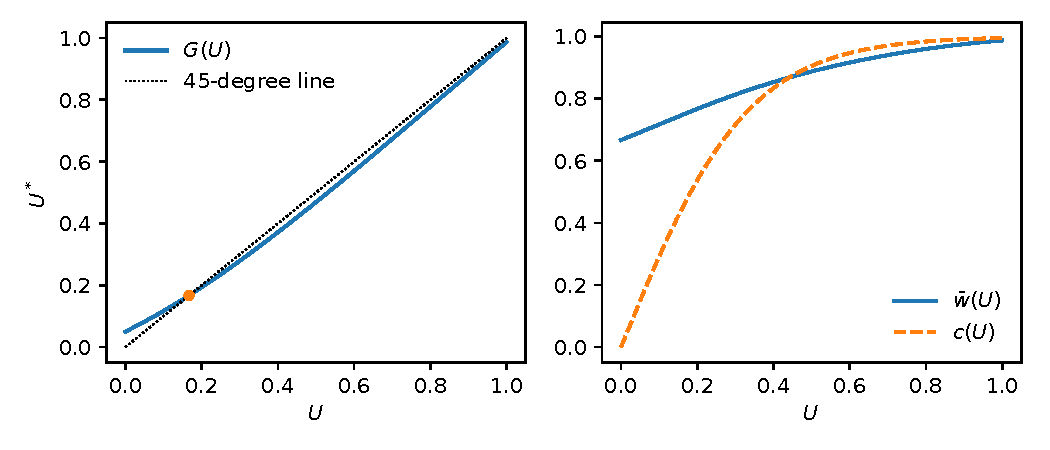
\includegraphics[width=0.9\linewidth]{fig/ls07_search.pdf}\\[3pt]
\captionof{figure}{Exercise 7.7. Left: the equilibrium law of motion $U^*=G(U)$. Right: the
reservation wage and the benefit schedule.}
\end{center}

\emph{Reading of the timing.} Under the stated timing, a worker hired this period is exposed to
firing at the start of the next one. Exact accounting would then give
$U^*=\lambda(1-U+\phi U)+(1-\phi)U$, but the book's law omits the term $\lambda\phi(U)U$. We take
the stated law as the definition of the aggregate dynamics, as the exercise directs. The individual
Bellman equations are unaffected. Under the alternative law the example's steady state would be
$U_s=0.1796$ instead of $0.1671$.

\begin{tcolorbox}[databox]
Independent route: the scalar steady-state equations (Brent's method) give $U_s$ and $\bar w_s$
equal to the grid RCE to $10^{-4}$. A sign-change count on $(0,1)$ confirms uniqueness, and a
simulated path of $U$ from $0.4$ converges to $U_s$.
\end{tcolorbox}
\end{tcolorbox}

%======================================================================
\section*{Companion code}
\addcontentsline{toc}{section}{Companion code}
%======================================================================

Every numerical result above is reproduced by the notebook \texttt{ls\_ch07.ipynb} in this folder
(executed, outputs saved). Each claim is checked by an independent route with an \texttt{assert}.

\begin{center}
\begin{tabular}{@{}lp{11.2cm}@{}}
\toprule
\textbf{Section} & \textbf{What it checks} \\
\midrule
Shared & \texttt{olrp}, \texttt{dare}, \texttt{evaluate}, \texttt{howard} copied from \texttt{ls\_ch05.ipynb}; new \texttt{nnash} (stacked Riccati). \\
7.1 & Return mapping; \texttt{olrp} vs DARE vs undetermined coefficients; Euler residual; actual law for $n$ firms. \\
7.2 & $\mathcal M(H)$ at pairs (i)--(iii); quadratic fixed point; Jacobian by finite differences; damped vs undamped algorithm; figure. \\
7.3--7.4 & Surplus by quadrature vs quadratic form; \texttt{olrp} vs DARE vs Euler closed forms; REE $=$ planner. \\
7.5 & \texttt{nnash} vs best-response iteration; DARE given the rival's rule; symmetry; steady state; figure. \\
7.6 & Grid backward induction (MPE and commitment) vs log/Cobb--Douglas closed form; welfare ranking; figure. \\
7.7 & Grid RCE vs scalar steady state; uniqueness; monotone $\bar w$, $G$; alternative timing; figure. \\
\bottomrule
\end{tabular}
\end{center}

Figures are saved to \texttt{fig/ls07\_*.pdf} with TrueType (not Type~3) fonts.

\end{document}
